\documentclass{article}

\title{Product Specification}
\author{Group 5}
\usepackage{outlines}
\usepackage{graphicx}
\graphicspath{{images/}{../diagrams/}}
\date{}

\begin{document}
    \maketitle
    
    \section{Description}
    The chess application will allow the user to play chess against another person locally, or against an AI which will have \\
    three different difficulties; easy, medium and hard. The application will also be able the track the results of the games and \\
    save the skill rating (using the Elo system) of the users and place them on a scoreboard. The AIs will be at a static rating \\
    for each difficulty level.
    
    \section{System Requirements} 
    \subsection{Functional:}
    \begin{outline}
          \1 Users shall be able to play against another human opponent (multiplayer).
          \1 The system shall appoint rankings to the players of the game, which indicates 
             that the winner of a game is awarded points which will have to be calculated.
          \1 The system keeps track of the results for each game played.
          \2 This enables the system to provide an overview of the ranking of the human participants,
             based on on how many games they have won.
          \1 Users shall be able to play against an AI, which will have 3 levels of difficulty:
          \2 Easy
          \2 Medium
          \2 Hard
          \1 Winning against a more intelligent or higher ranked AI should award more points.
     \end{outline}
     
    \subsection{Non-functional:}
    \begin{outline}
          \1 The system shall be made with 2D graphics.
          \2 It must feature a board layout.
          \2 It must feature player statistics.
          \1 The system shall be implemented on top of a open source graphics engine.
          \2 The game shall be implemented in JavaFX.
          \1 The system shall be programmed in such a way that the ruleset (board size etc.) can easily be changed.
          \1 System shall be programmed in Java.
    \end{outline}
    
    \section{User stories}
        USER STORY 1: As a Chess player I want to play against good chess AI’s 
        so I can become better at chess. \\
        
        \noindent
        USER STORY 2: As a pair of friends, we want to play chess together so we
        can spend more time with each other. \\
        
        \noindent
        USER STORY 3: As a user of the chess game I want my available moves to 
        be visualized when I pick a given chess-piece. \\
        
        \noindent
        USER STORY 4: As a beginner level chess player I want to learn to play 
        the game/basic rules of the game so I can play the game without help. \\
        
        \noindent
        USER STORY 5: As a user I want the moves I make to be viewable through 
        the course of a game. \\
        
        \noindent
        USER STORY 6: As a frequent user of the software i want my MMR to be 
        saved/updated after every match so i can show it to my friends. \\
	
	\vspace{30mm}
    \section{Use case diagram}
    Diagram showcasing the major user operations of the chess application. \\ \\
    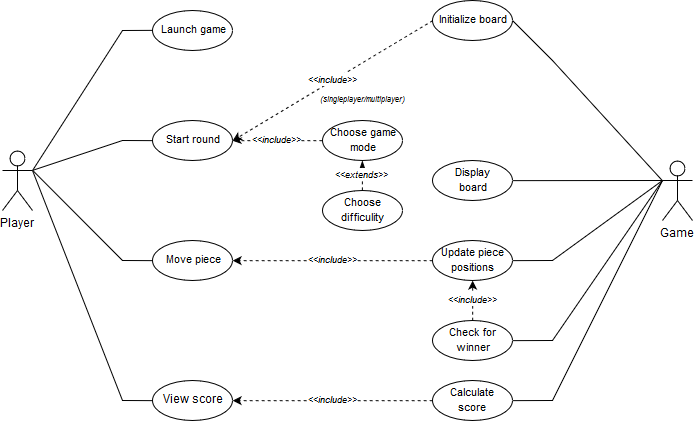
\includegraphics[scale=0.6]{usecase-diagram.png}
    
    \vspace{100mm}
    \section{Use cases}
        \subsection{Use case 1 (fully dressed)}
        A start menu allows a user to start the game and choose single player to
        play against a machine AI. The user will be prompted to write their player
        name so the high score can be saved in an external file. In the next step
        the player has to choose between three difficulties. After the AI difficulty
        is chosen, the game will start. The player must progress by moving their
        pieces according to the game rules. The player can move pieces by clicking
        on their piece (if it is their turn and a legal move) and pick the square that
        the piece should be moved to. The machine will respond according to the 
        difficulty chosen by the player earlier. \\ \\
        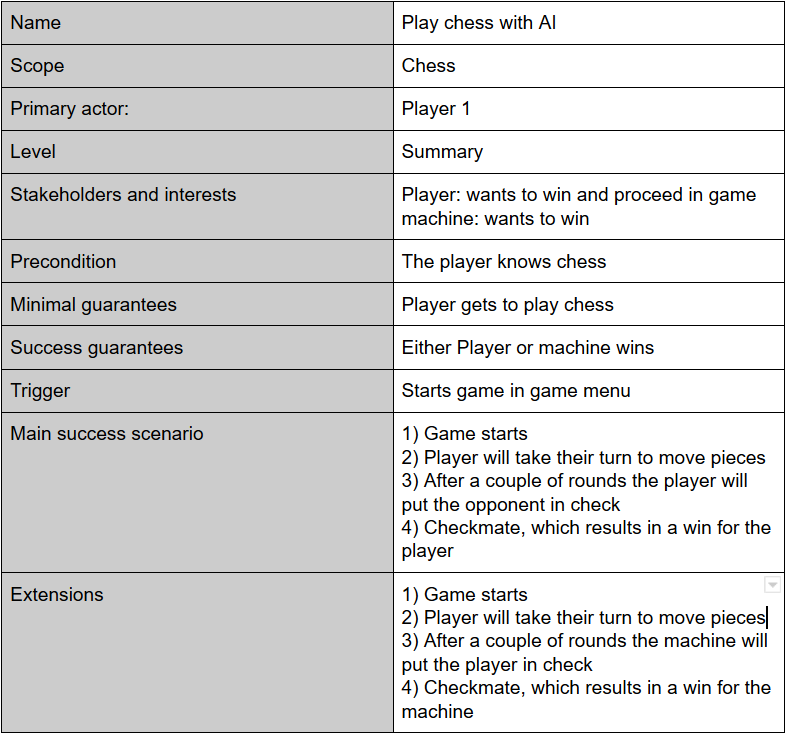
\includegraphics[width=\linewidth]{play-ai.png}
        
        \vspace{30mm}
        \subsection{Use case 2 (fully dressed)}
        A start menu allows a user to start a game and choose multiplayer with 
        another local player. After the player picks the multiplayer option it 
        will be prompted to write name of player 1, then name of player 2, so 
        the high score can be saved in an external file. After the name dialog,
        the players will be taken to the chess game and the possibility to play
        against each other. The game will be started and either player 1 or 2 starts.
        The players must progress with moving their pieces according to the game rules.
        The player can move pieces by clicking on their piece (if it is their 
        turn and a legal move) and pick the square that the piece should be moved
        to. \\ \\
        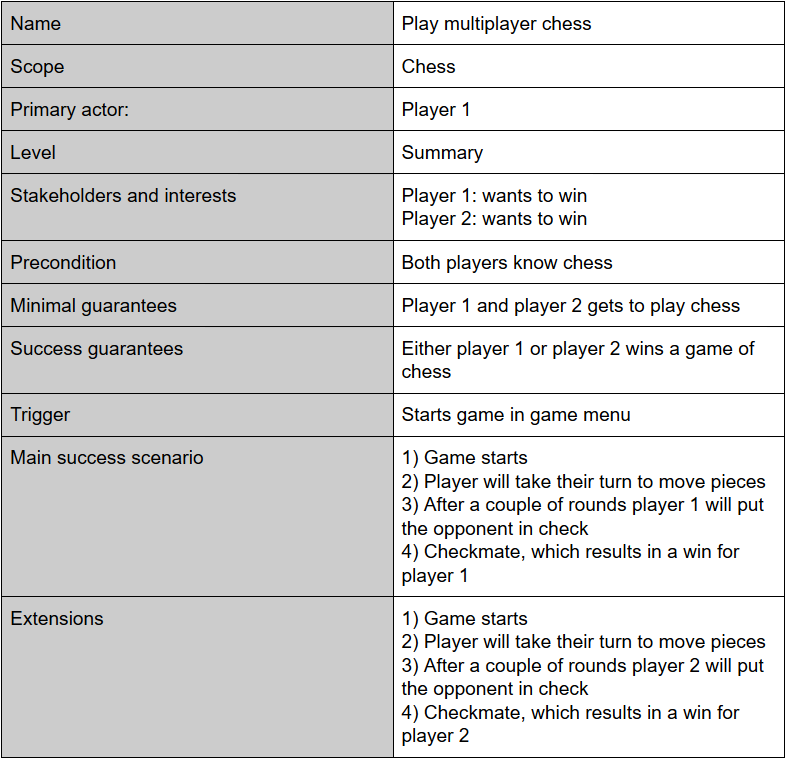
\includegraphics[width=\linewidth]{play-multiplayer.png}
        
    \section{Domain model (class diagram)}
    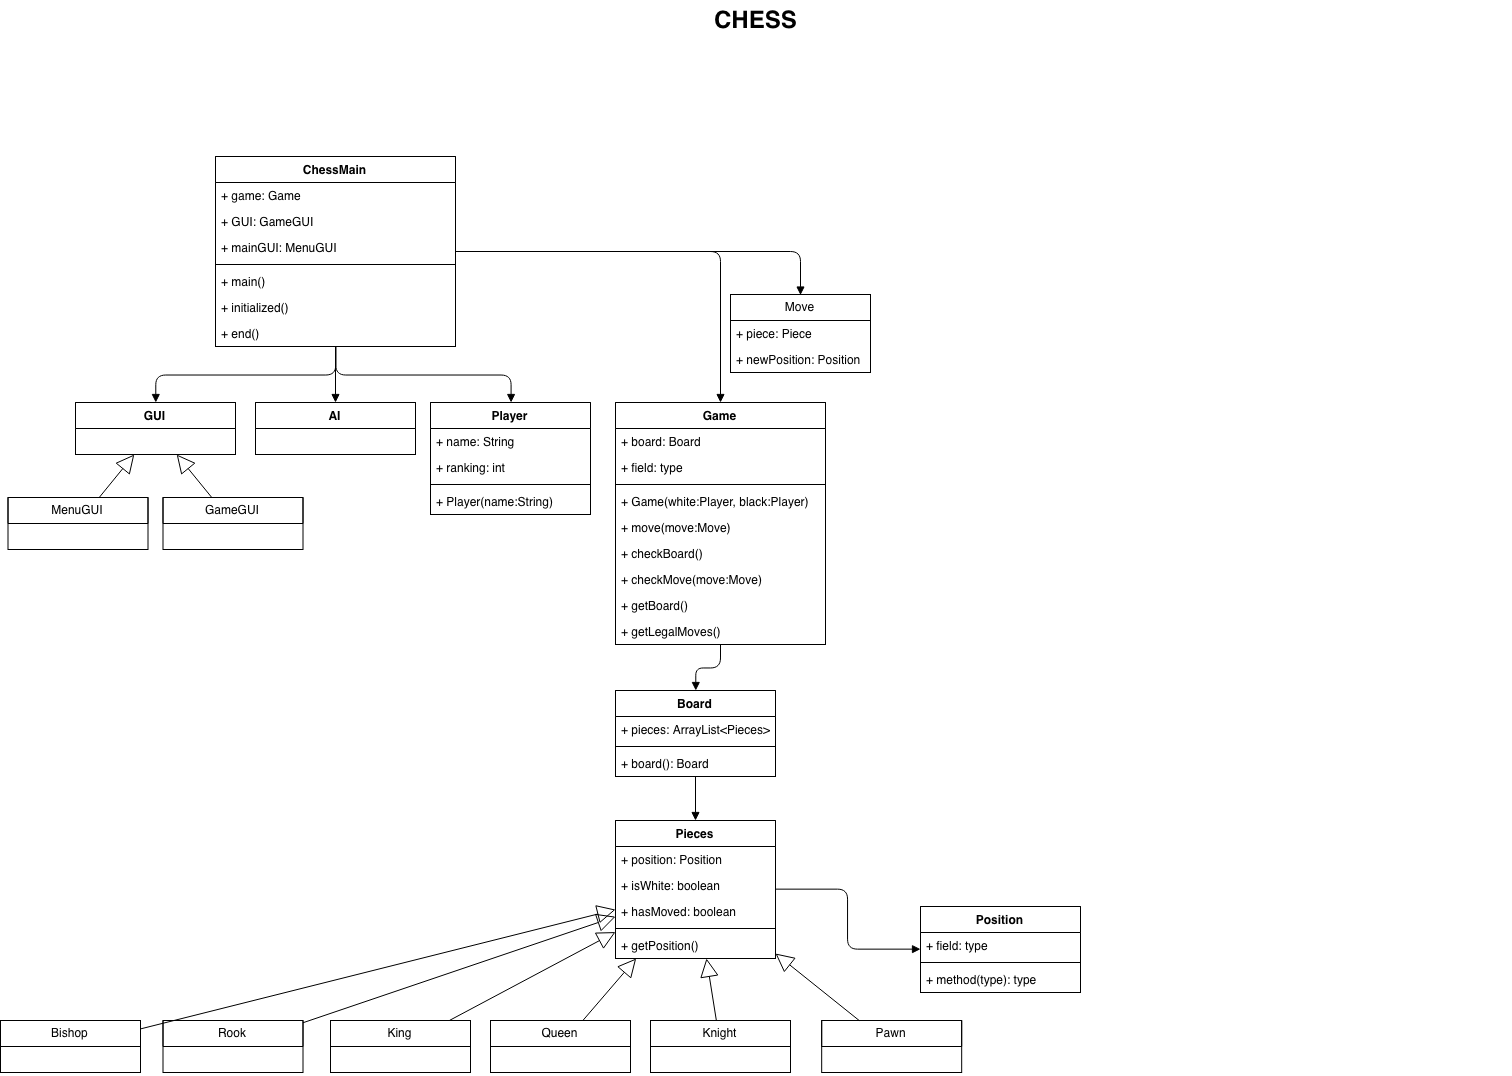
\includegraphics[scale=0.35]{class-diagram.png}
    
    \subsection{Short explanation of the project structure}
    	The ChessMain class is in charge of showing the board to the player and update it according to user input.
	Here we make a Board object that we display to the user with the help of the javafx library.
	We get user input that we can use to change the board, or alternately we can get input from the AI.
	Whenever we change the board we also draw the new board for the user to see. 
	All of this is taken care of in the ChessMain class.
	The actual game logic is all taken care of in the Board class.
	It will keep track of the two players as well as all the tiles that can contain a piece.
	Tile is a way of keeping track of all the pieces in a way that makes is easy to draw in the GUI.
	The pieces contain all the logic of how they can move,
	so we can simply call that piece to get its possible moves.
	The Player contain information necessary to analyze the board for certain events.
	It is also capable of making a move 
	which means returning a new board object similar to the one it belongs to just with the move done.
	Remember all of these are reachable from Board and thus ChessMain.
    There are several helper classes, factories and enums left out of this graph to make it readable, but this is the overall structure off the entire project.

\end{document}
